\documentclass[a4paper, 12p]{article}
\usepackage[spanish]{babel} 
\usepackage{amsmath} 
\usepackage[colorlinks=true]{hyperref}
\usepackage{enumitem} 
\usepackage{graphicx}   
\usepackage[a4paper,top=3cm,bottom=3cm,left=3cm,right=3cm,marginparwidth=1.75cm]{geometry} 
\usepackage[]{subfigure}
\graphicspath{{./graficos/Lab-Termo/Git/Documentos}} 
\usepackage{float}
%\usepackage[]{txfonts}
\usepackage{multicol}



\newenvironment{Figura}
{\par\medskip\noindent\minipage{\linewidth}}
{\endminipage\par\medskip}

%==================================================================================
\begin{document}
\begin{titlepage}
      \begin{center}     
              
            
\includegraphics[width=0.2\textwidth]{imag/escudo_udec.png}                       %Para poner logo udec   %{nombre carpeta\nombreimagen}
            
            
            
            \vspace{1cm}
            \textsc{{\LARGE Universidad de Concepción}}
            
            \vspace{1cm}
            {\scshape\Large Facultad de ciencias fisícas y matemáticas \par}
            \vspace{2cm}
            {\scshape\Huge Laboratorio 2 \par}
            \vspace{2cm}
            {\itshape\Large Proyecto laboratorio termodinámica \par}
            \vfill
            {\Large Autores: \par}
            {\Large Martina Contreras, Noemí De la peña, Benjamín Opazo. \par}
            \vfill
            \vfill
            {\Large Profesor: \par}
            {\Large Claudio Alonso Faúndez Araya \par}
            \vfill
            \vfill
            {\Large Carrera: \par}
            {\Large Ciencias fisícas \par}
            \vfill
            \vfill
            {\Large Ayudantes: \par}
            {\Large Arelly Nunez y Anahis Verana \par}
            \vfill
            {\Large Octubre 2022 \par}
      \end{center}
\end{titlepage}            
%\maketitle  

\tableofcontents
\newpage

%========Introducción
\section{Introdución}
Presentaremos en este informe datos obtenidos del simulador de laboratorio, del cual debimos anotar en una tabla la temperatura de 3 diferentes sustancias para 4 experiencias distintas. Además mostraremos las curvas de calentamientos , los puntos de fusión y ebullición, los calores latentes de fusión y de ebullición, de cada sustancias.
En donde primero definiremos, que es un calor latente de fusión y de ebullición, también diremos como se relacionan estas con la masa, temperatura inicial y el calor. Para luego exponer los materiales utilizados para el laboratorio, además del procedimiento seguido para realizarlo.
Los datos serán presentados tanto en tablas como en gráficas, de las cuales obtendremos información con la que responderemos las preguntas propuestas. 
Por último, diremos si se logro cumplir los objetivos de este laboratorio y diremos si nuestra hipótesis planteada fue correcta o incorrecta.

\section{Objetivos}
\begin{itemize}
      \item Determinar experimentalmente las curvas de calentamiento de diferentes sustancias.
      \item Determinar los puntos de fusión y de ebullición de diferentes sustancias.
      \item Estudiar algunos factores que intervienen en el calentamiento de una sustancia.
      \item Determinar calores latentes de fusión y de ebullición.
\end{itemize}




%=========Marco Teórico
\section{Marco Teórico} 

\begin{itemize}
      \item \textbf{Capacidad calorífica: }(a cualquier temperatura) se define como  el limite de C cuando $\varDelta T$ tiende a 0:
      \begin{align}
            C = \frac{d'Q}{dT}           \qquad \left[\frac{J}{K}\right]              
      \end{align}
      donde: \\ \\
      $d'Q = $ Representa un pequeño flujo de calor. \\
      $dT = $ Es el correspondiente al cambio de temperatura. 

      \item \textbf{Calor específico: } Capacidad calorífica por unidad de masa o mol.
      \begin{align}
            c = \frac{C}{n}   \quad \left[\frac{J}{Kilo\cdot molK}\right]  \qquad o  \qquad c = \frac{C}{m} \quad \left[\frac{J}{KgK}\right]
      \end{align}

      \item \textbf{Cantidad total de calor } que fluye en un sistema en cualquier proceso, viene dado por:
      \begin{align}
            Q = \int d'Q &= \int_{T_i}^{T_F} C\cdot dT \\ \nonumber
                         &= \int_{T_i}^{T_F} mc\cdot dT
      \end{align}
      cuando c es constante, obtenemos que:
      \begin{align}
            Q = mc \, \varDelta T
      \end{align}

      \item \textbf{Calor latente o de transformación: } Es la razón del calor absorbido a la masa m que experimenta el cambio de fase. 
      \begin{align}
            l = \frac{Q}{m}                \qquad \left[\frac{J}{Kg}\right]
      \end{align}
      donde: \\ \\
      $Q$ = Es el flujo de calor necesario para que exista un cambio de fase.\\
      $n$ = moles

      \item \textbf{Cambio de fase: } se refiere a que una sustancia que absorve o cede calor sin que haya un cambio en su temperatura.
      \item \textbf{Calor latente de fusión: }es el calor requerido por unidad de masa para cambiar de un estado sólido a líquido a una presión y temperatura fija.
      \item \textbf{Calor latente de evaporación: } es el calor requerido por unidad de masa para pasar de un estado líquido a gaseoso a una presión y temperatura fija.
\end{itemize} 
Cada concepto fue extraído de \cite{libro}. \\

Nuestras hipótesis son:
\begin{enumerate}
      \item A mayor cantidad de sustancia, mayor será el tiempo en el que alcance el punto de ebullición.
      \item  A mayor potencia, la sustancia alcanza más rápido su punto de ebullición.
      \item A mismas condiciones iniciales, diferentes sustancias pueden alcanzar su punto de ebullición en distintos intervalos de tiempo.
      
      
\end{enumerate}







%=========Materiales
\section{Materiales}


\begin{itemize}
      \item Termómetro digital
      \item Vaso precipitado
      \item Estufa eléctrica 
       \item Agua
      \item Alcohol etílico
      \item Benceno
\end{itemize}




\begin{figure}[H]
      \begin{subfigure}
            \raggedleft
            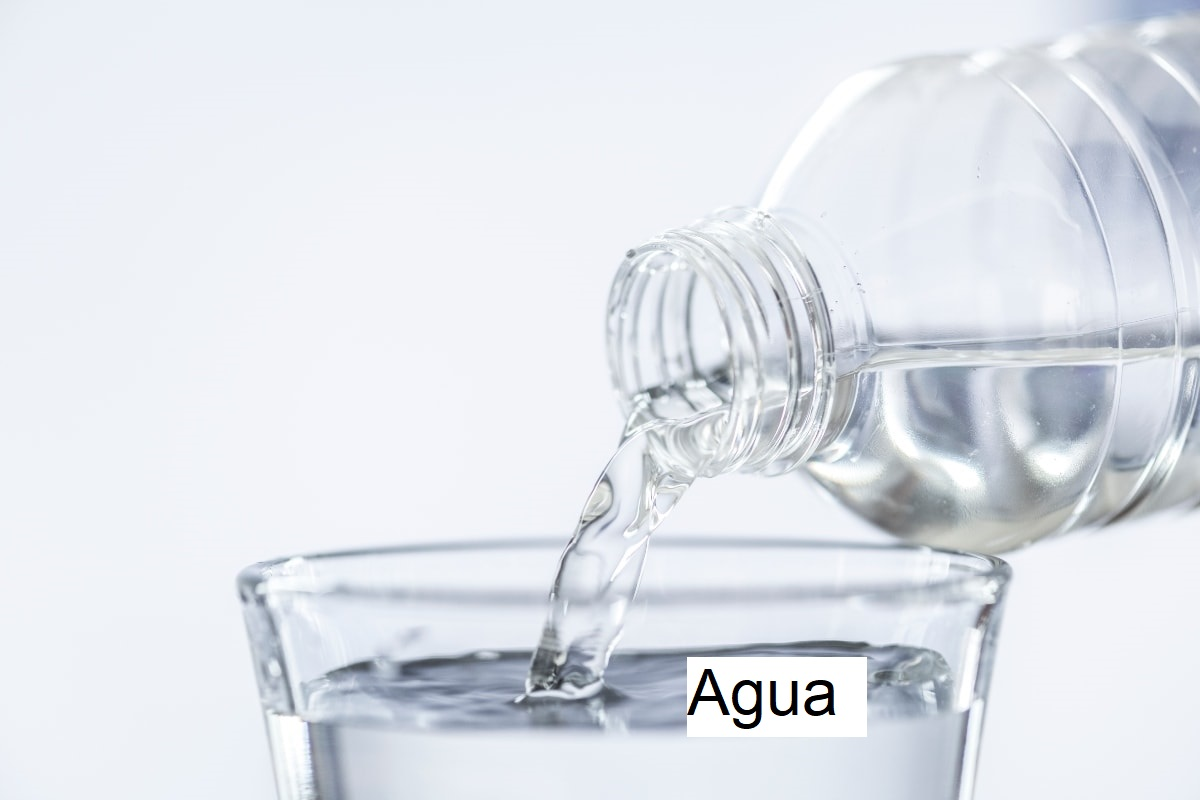
\includegraphics[width=4cm, height=4cm]{imag/agua.jpg}
      \end{subfigure}
      \begin{subfigure}
            \raggedleft
            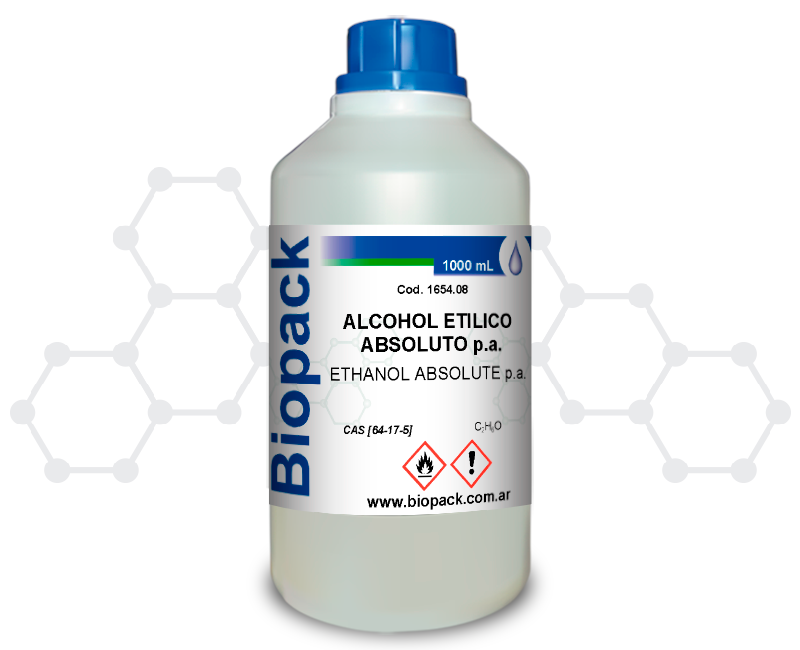
\includegraphics[width=4cm, height=4cm]{imag/alcohol.jpg}
      \end{subfigure}
      \begin{subfigure}
            \raggedleft
            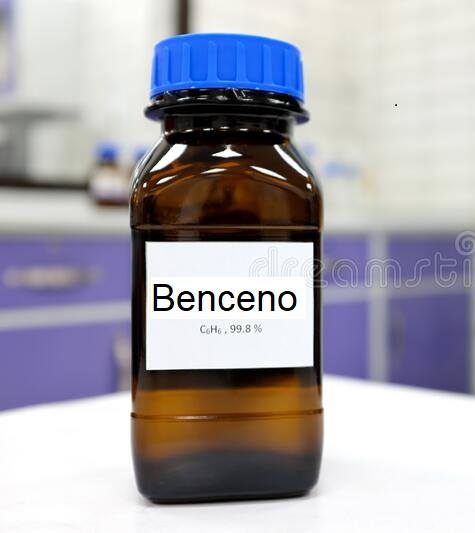
\includegraphics[width=4cm, height=4cm]{imag/benceno.jpg}   
      \end{subfigure}   
      \begin{subfigure}
            \raggedleft
            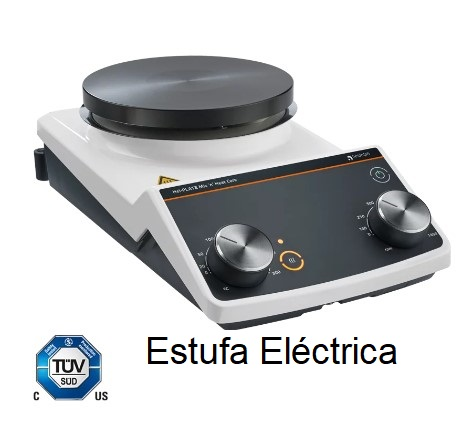
\includegraphics[width=4cm, height=4cm]{imag/estufa.jpg} 
      \end{subfigure}
      \begin{subfigure}
            \raggedleft
            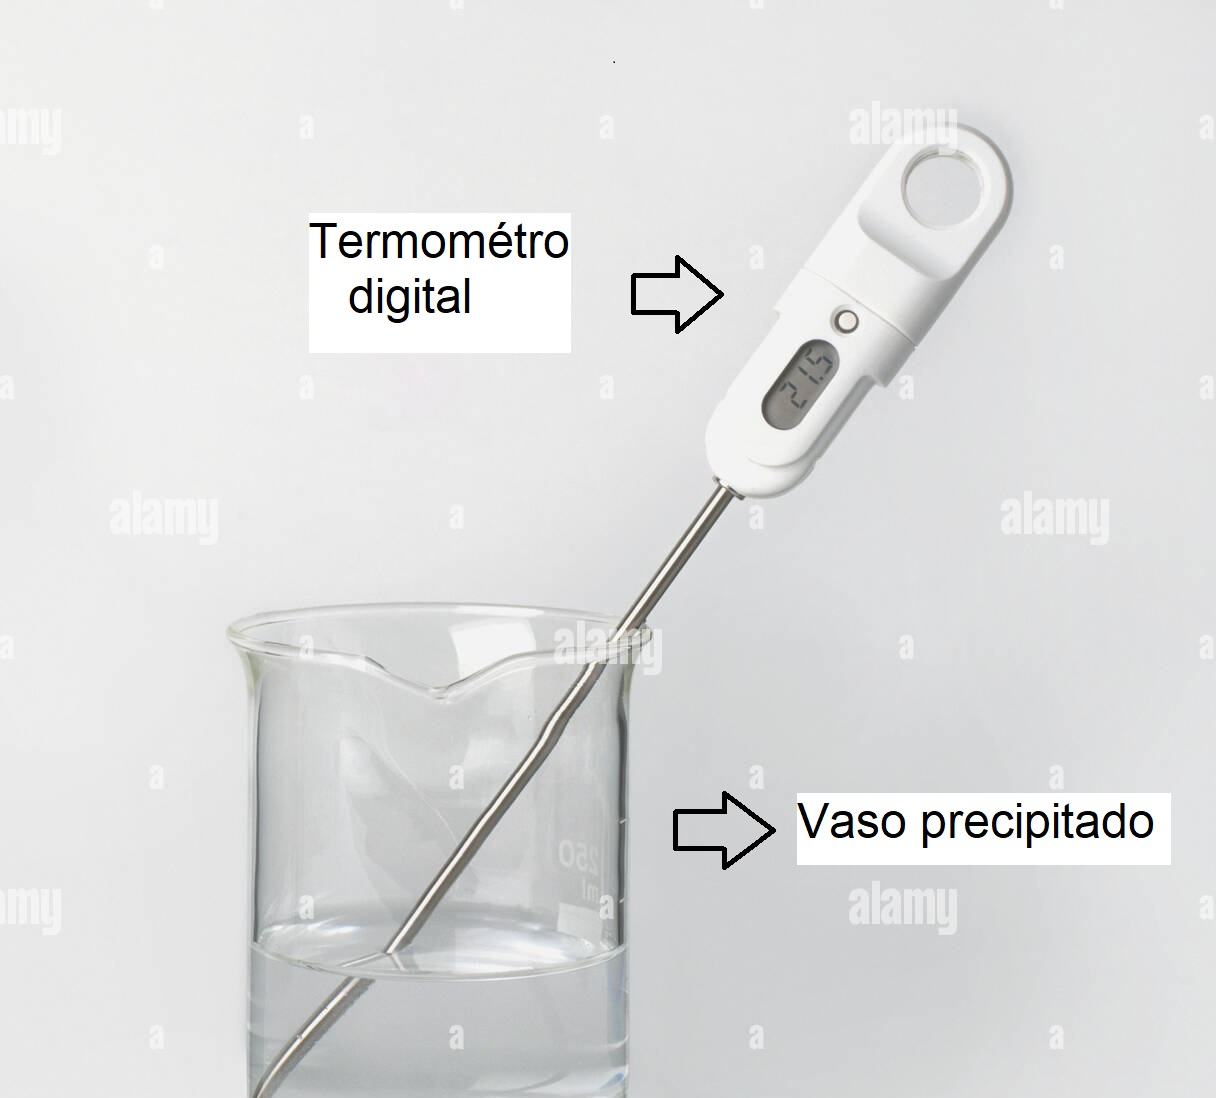
\includegraphics[width=5cm, height=4cm]{imag/termometro.jpg} 
      \end{subfigure}
\end{figure}     









\section{Procedimiento y Resultados}


\subsection{Determinación puntos de fusión y de ebullición}
\begin{itemize}
      \item Primero, seleccionaremos una potencia de 250 [W], una masa de 150[g] de agua y una temperatura inicial de -10°C.
      \item Segundo, anotamos la temperatura, hasta llegar al punto de ebullición.
      \item Tercero, realizamos lo mismo para el alcohol y el benceno.
      \item Finalmente, hacemos un gráfico de temperatura vs tiempo para los datos obtenidos.
\end{itemize}


\begin{table}[H]
      \centering
      \begin{tabular}{|c|c|c|}\hline
            Sustancia [g]& Tiempo [s] & Temperatura [°C]\\ \hline
                          &    0     &  0\\
                          &     1.7  & -8.6\\
                          &   30.9   & 0\\
                          &   60.1   & 0\\
                          &   93.7   & 0\\
                          &   99.1   & 0\\
                          &   120.1  & 0\\
                          &   149.8  & 0\\
             agua         &   180.2  & 0\\
                          &   209.9  & 0\\
                          &   240.3  & 10.9\\
                          &   269.7  & 22.6\\
                          &   300.2  & 34.7\\
                          &   329.9  & 46.6\\
                          &   360.0  & 58.5\\
                          &   389.9  & 70.5\\
                          &   419.9  & 82.4\\
                          &   450.5  & 94.6\\
                          &   480.1  & 100\\ \hline
                          &0.0       &-10.0\\
                          &30.3      &10.5\\
           alcohol        &60.1      &30.7\\
                          &89.9      &50.9\\
                          &120.1     &71.3\\
                          &150.3     &78.3\\ \hline
                          &0.0      &-10\\
                          &18.0     &5.5\\
                          &30.1     &5.5\\
           benceno        &60.3     &5.5\\
                          &90.1     &5.5\\
                          &121.1    &31.5\\
                          &149.8    &58.9\\
                          &172.8    &80.2\\ \hline
      \end{tabular}
      \label{tab: fusion-ebullicion}
      \caption{Datos de experimento:  ebullición - fusión.} 
\end{table}

\begin{figure}[H]
      \centering
      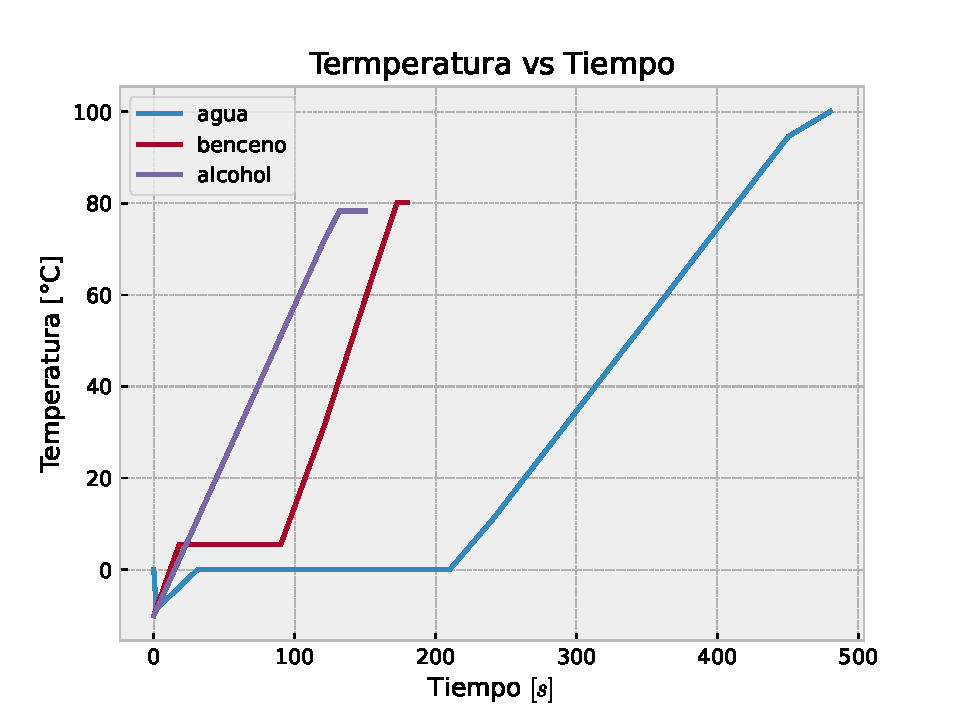
\includegraphics[width=12cm, height=8cm]{ebullicion-fusion/grafico-ebullicion-fusion.pdf}
      \label{img: ebullicion-fusion}      
\end{figure}


\begin{table}[H]
    \centering
 \begin{tabular}{|c|c|c|c|}\hline
                            &  agua &  alcohol  &   benceno  \\ \hline
 Punto de fusión (°C)       &   0   &  N/A      &    5.5      \\ \hline
 Punto de ebullición (°C)   &   100 &    78.3   &    80.2      \\ \hline
    
 \end{tabular}
 \label{tab:ebullicion-fusion2} 
 \caption{ Puntos de fusión y de ebullición.}
\end{table}



\subsection{Masa de una sustancia}
\begin{itemize}
      \item Primero, seleccionaremos una potencia de 500[W], una masa de 100[g] 
      de alcochol y una temperatura inicial de 10°C.
      \item  Segundo, anotaremos la temperatura, al menos 8 valores espaciados. El punto de ebullición no será considerado.
      \item Tercero, repetiremos el experimento para 150[g] y 200[g] de alcohol.
\end{itemize}
Según los datos obtenidos \ref{img: masa} mientras menor sea la masa de la sustancia, más rápido se calentará.

\begin{table}[H]
      \centering
      \begin{tabular}{|c|c|c|}\hline
           Masa [g]& Tiempo [s] & Temperatura [°C]\\ \hline
                   &   0.0      &  10.0\\
                   &   5.1      &  20.3\\
                   &   9.8      &  29.9\\
          100      &   14.3     &  39.0\\
                   &   18.4     &  47.3\\
                   &  22.9      &  56.5 \\
                   &  27.3      &  65.4\\
                   &  31.7      &  74.4\\ \hline
                   & 0.0        &  10.0\\
                   &4.1         &  15.5\\
                   &7.9         &  20.7\\
                   &11.0        &  24.9\\
                   &14.7        &  29.9\\ 
          150      &18.5        &  35.0\\
                   &22.0        &  39.8\\
                   &25.2        &  44.1\\
                   &29.1        &  49.4\\
                   &32.7        &  54.3\\
                   &36.7        &  59.7\\
                   &40.5        &  64.8\\
                   &44.5        &  70.2\\
                   &48.1        &  75.1\\ \hline 
                  &    0.0       &10.0\\
                  &   4.9        &14.9\\
                  &    8.3       &18.4\\
                  &    11.2      &21.3\\
                  &    14.9      &25.1\\
                  &    18.4      &28.6\\
                  &    21.7      &32.0\\
                  &   25.2       &35.6\\
                  &    29.1      &39.5\\
      200         &    33.1      &43.6\\
                  &    36.9      &47.5\\
                  &    41.3      &51.9\\
                  &    44.9      &55.6\\
                  &    50.3      &61.1\\
                  &    53.3      & 64.1\\
                  &    57.3      & 68.2\\
                  &    61.1      &72.0\\
                  &    64.9      &75.9\\ \hline
      \end{tabular}
      \label{tab:masa }
      \caption[]{Datos del experimento: Masa de una sustancia.}
\end{table}

\begin{figure}[H]
      \centering
      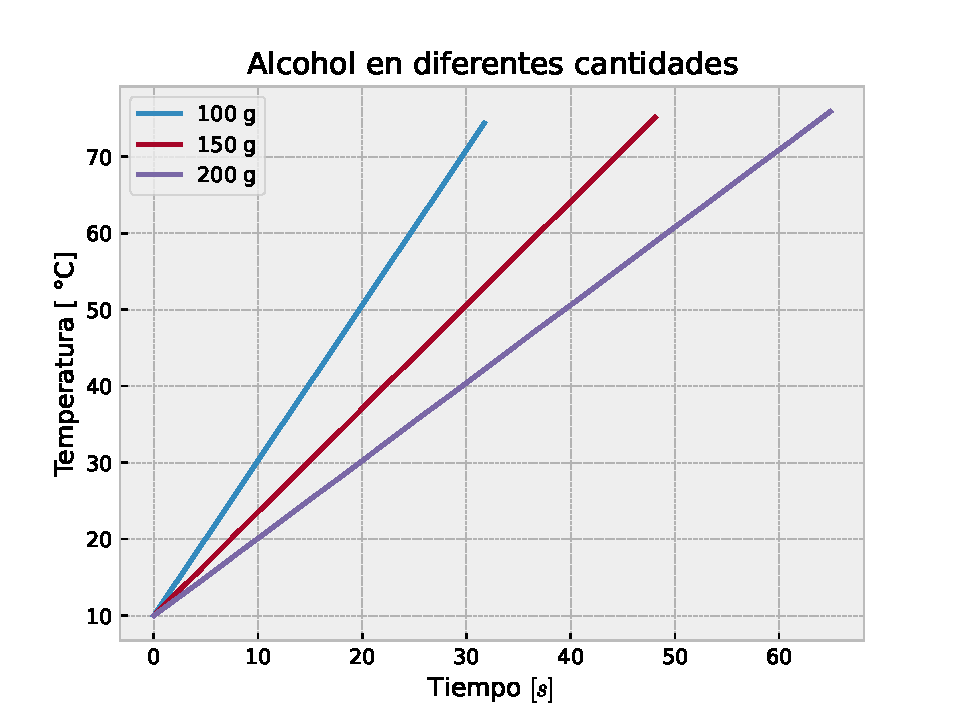
\includegraphics[width=12cm, height=8cm]{masa/grafico-alcohol-masa.pdf}
      \label{img: masa}
\end{figure}



\subsection{Potencia de la estufa}
\begin{itemize}
      \item Primero, seleccionaremos una potencia de 250[W], una masa de 100[g] de benceno y una temperatura inicial de 10°C.
      \item Segundo, anotaremos la temperatura, al menos 8 valores espaciados. El punto de ebullición no será considerado.
      \item Tercero, repetiremos el experimento para 500[W] y 1000[W].
\end{itemize}
Segun los datos obtenidos \ref{img: potencia} a mayor potencia, la sustancia alcanza más rápido su punto de ebullición.


\begin{table}[H]
      \centering
      \begin{tabular}{|c|c|c|}\hline
            Potencia [W]& Tiempo [s] & Temperatura [°C]\\ \hline
                        &   0.0    &10.0\\
                        & 3.7      &15.2\\
                        &8.1        &21.5\\
                        &11.5       &26.4\\
                        &15.7       &32.4\\
            250         &19.4       &37.7\\
                        &22.9        &42.7\\
                        &26.7        &48.1\\
                        &31.1         &54.4\\
                        &35.1         &60.1\\
                        &39.5         &66.4\\
                        &43.7        &72.4\\
                        &48.1        &78.7\\ \hline        
                        &0.0         &10.0\\
                        &3.1        &18.8\\
            500         &6.5        &28.5\\
                        &10.0       &38.5\\
                        &13.1       &47.4\\
                        &16.9       &58.2\\
                        &19.9       &66.8\\
                        &23.0       &75.7\\ \hline
                        &0.0        &10.0\\
                        &1.7        &19.7\\
            1000        &3.3        &28.8\\
                        &4.9        &38.0\\
                        &6.5         &47.1\\
                        &7.9        &55.1\\
                        &9.2         &62.5\\
                        &10.3       &68.8\\
                        &11.5       &75.7\\ \hline    
      \end{tabular}
      \label{tab: potencia}
      \caption[]{Datos del experimento: Potencia de la estufa.}
      
\end{table}
\begin{figure}[H]
      \centering
      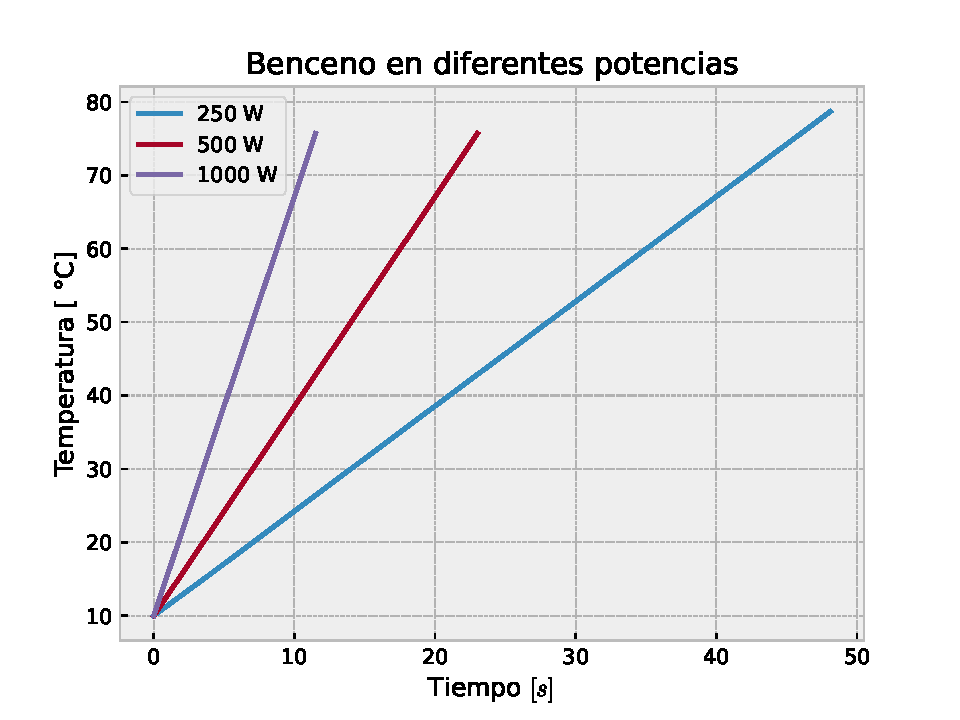
\includegraphics[width=12cm, height=8cm]{potencia/grafico-benceno-potencia.pdf}
      \label{img: potencia}
\end{figure}



\subsection{La naturaleza de la sustancia}
\begin{itemize}
      \item Primero, seleccionaremos una potencia de 250[W], una masa de 150[g] de agua a una temperatura inicial de 0°C.
      \item Segundo, anotaremos la temperatura, al menos 8 valores espaciados. El punto de ebullición, no será considerado.
      \item Tercero, repetiremos el experimento para la sustancia de alcohol y benceno.
\end{itemize}
Según los datos obtenidos \ref{img: naturaleza} el alcohol, a mismas condiciones iniciales, se demora menos en alcanzar su punto de ebullición.

\begin{table}[H]
      \centering
      \begin{tabular}{|c|c|c|}\hline
            Sustancia [W]& Tiempo [s] & Temperatura [°C]\\ \hline
                            &  0.0  &0.0\\
                            & 29.9  &0.0\\
                            & 59.7  &0.0\\
                            & 90.1  &0.0\\
                            & 119.9 &0.0\\
                            & 149.7 &0.0\\
                            & 179.8 &0.0\\
         agua               & 210.3 &3.9\\
                            & 239.9 &15.6\\
                            & 269.9 &27.6\\
                            & 300.0 &39.6\\
                            & 330.0 &51.5\\
                            & 359.9 &63.4\\
                            & 389.9 &75.4\\
                            & 419.5 &87.2\\
                            & 450.3 &99.5\\ \hline
                              & 0.0  & 0.0\\
                              & 14.7 & 9.9\\
                              & 29.9 & 20.2\\
         alcohol              & 45.1 & 30.5\\
                              & 59.9 & 40.5\\
                              & 74.7 & 50.6\\
                              & 89.9 & 60.9\\
                              & 104.7 & 70.9 \\ \hline
                              &0.0  &0.0\\
                              &19.5 &5.5\\
                              &39.7 &5.5 \\
        benceno               &60.1 &5.5\\
                              &79.9 &5.5\\
                              &99.7 &21.8\\
                              &120.1 &41.3\\
                              & 139.8 &60.0\\
                              &159.7 &79.0\\ \hline

      \end{tabular} 
      \label{tab: naturaleza}
      \caption[]{Datos del experimento: La naturaleza de la sustancia.}
\end{table}


\begin{figure}[H]
      \centering
      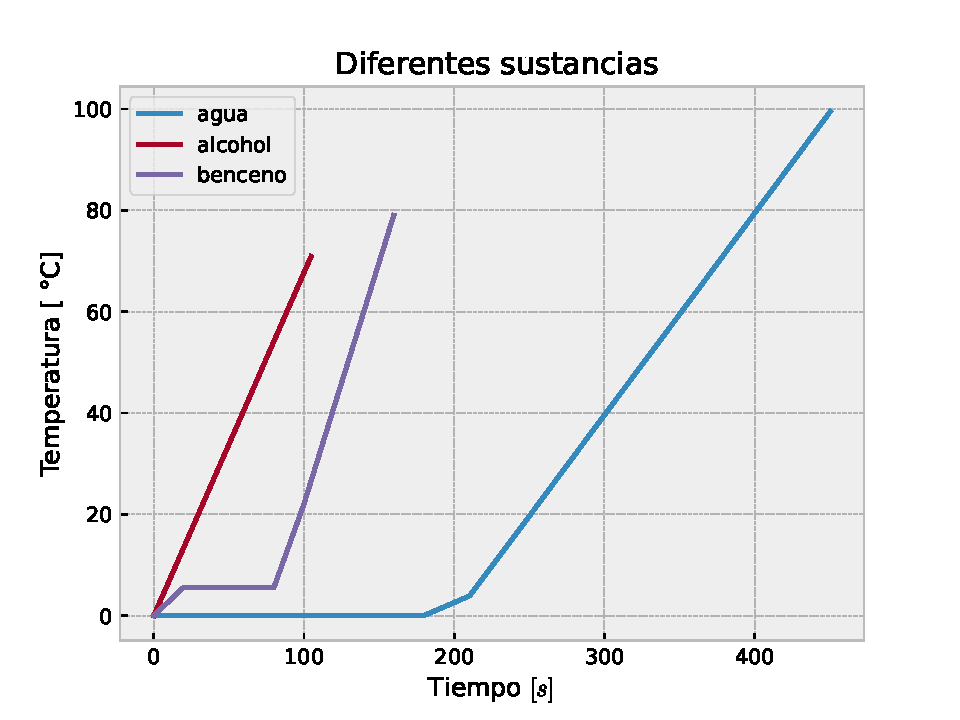
\includegraphics[width=12cm, height=8cm]{naturaleza/grafico-naturaleza-sustancias.pdf}
      \label{img: naturaleza}
\end{figure}

\section{Análisis}
\begin{enumerate}
	\item ¿Qué es el calor latente de fusión y evaporación?\\
		  R: El calor latente de fusión es el calor requerido por unidad de masa para cambiar de un estado sólido a líquido a una presión y temperatura fija, similarmente, el calor latente de evaporación es el calor requerido por unidad de masa para pasar de un estado líquido a gaseoso a una presión y temperatura fija.\\
	\item Un calorímetro contiene 220 ml de agua a 55ºC y 27 g de hielo a 0ºC. Determine la temperatura final del sistema.Sea $L_{f} = 3.33x10^2 J/g$, el calor latente de de fusión del hielo.\\ \\
		  R: Nuestros datos son\\ 
		     $m_{a} = 220 m$\\
		     $m{H} = 27 g$\\
		     $Ti_a$ = 55ºC , temperatura inicial del agua. \\
		     $Ti_H$ = 0ºC, temperatura inicial del hielo. \\ 
		     $L_{f} = 3.33 x 10^2 J/g$, calor latente de fusión del hielo.\\
		     $c_{a}$ = 4.1813 J/gºC , calor especifíco del agua.\\
		     
		     Primero como el agua está a mayor temperatura que el hielo, la agua será la que cede calor y el hielo el que absorbe calor,\\ 
		     como el agua esta en ml, tenemos que convertir los ml a g, donde podemos usar la relacion $\rho = m/V$, donde $\rho$ es densidad, donde m es masa y V es el volumen, donde la densidad del agua, es aproximadamente $1g/ml$, de aquí tenemos que 1g de agua es igual a 1ml.\\
		     El calor del agua viene dado por:\\
		      
		     $Q_{a} = \int_{Ti}^{Tf} \!dQ \, dt  = \int_{Ti}^{Tf} \! mc \Delta T \, dt = c_{a} m_{a} \Delta T $, \\ 
		     
		     y el calor del hielo viene dado por:\\ 
		     
		     $Q_{H} = m_{H}L_{f} + m_{H}c_{a} \Delta T $,\\
		     
		     ,donde $m_{H}L_{f}$ corresponde al calor requerido para pasar de estado sólido, el hielo, a estado líquido, agua y $m_{H}c_{a} \Delta T$ corresponde al calor requerido para pasar de la temperatura que tiene el hielo derretido de 0ºC a $T_{f}$.\\
		     
		     Como el agua está a mayor temperatura que el hielo, la agua será la que cede calor y el hielo el que absorbe calor y por el principio de conservación de la energía tenemos que,\\
		     \begin{equation}\label{eq1}
		     m_{H}L_{f} + m_{H}c_{a} \Delta T = -(c_{a} m_{a} \Delta T),
		     \end{equation} 
		     
		     reemplazando nuestros datos en \ref{eq1} tenemos que,
		     \begin{equation}\label{eq2}
		     27 g \times 3.33 \times 10^2\dfrac{J}{g} + 27 g \times 4.1813\dfrac{J}{gºC}(T_{f} - 0ºC) = -(4.1813\dfrac{J}{gºC} \times 220 g(T_{f} - 55ºC))
		     \end{equation}
		     
		     resolviendo \ref{eq2} tenemos que,
		     
		     $T_{f}$ = 40.282ºC
		     
		  \item ¿Cuánto calor debe agregarse a 22 g de aluminio a 37ºC para fundirlo completamente?.Sea $c_{Al} =$ 0,9JºC el calor específico del aluminio y $L_{f} = 397J/g$, el calor latente de fusión del aluminio.
Nota:Buscar el punto de fusión del aluminio.\\
		  R: Nuestros datos son:\\
		  
		     $m_{al} = 22g$ \\
		     $c_{al}$ = 0.9J/gºC, el calor especifíco del aluminio \\
		     $T_{i}$ = 37ºC, temperatura inicial del aluminio \\
		     $T_{f}$ = 660.3ºC \\
		     $L_{f}$ = 397J/g, calor latente de fusión del aluminio \\  
		     
		     Sabemos que la temperatura de fusión del aluminio es 660.3ºC.\\
		     El calor total será el calor requerido para pasar el aluminio de 37ºC a 660.3ºC más el calor requerido para pasar el aluminio a 660.3ºC de estado sólido a estado líquido, al igual que la pregunta anterior $\int_{Ti}^{Tf} \!dQ \, dt  = \int_{Ti}^{Tf} \! mc \Delta T \, dt =  m_{al}c_{al} \Delta T $ con esto tenemos que
		     \begin{equation}\label{eq3}
		     Q_{al} = m_{al}c_{al} \Delta T + m_{al}L_{f}  
		     \end{equation}
		     
		     reemplazando en \ref{eq3} nuestros datos, tenemos que 
		    \begin{equation}\label{eq4}
		    Q_{al} = 22 g \times 0.9\dfrac{J}{gºC}(660.3ºC - 37ºC) + 22 g \times 397\dfrac{J}{g}
		    \end{equation}
		    
		    Resolviendo \ref{eq4} obtenemos que,\\
		   
		    $Q_{al} = 21075.34 J$
		    
\end{enumerate}



\section{Conclusión}
Al finalizar el informe, podemos decir que los objetivos se cumplieron. Se logro graficar las curvas de calentamiento de cada sustancia, determinamos tantos los puntos de fusión y de ebullición como el calor latente de fusión y 
de ebullición para cada sustancia, además de comprender que la masa, la temperatura inicial y el calor, tienen relación directa con la velocidad con la que llegan las sustancias a sus puntos de ebullición y fusión, de esta forma 
corroborando de manera experimental la ecuación de calor latente. \\
A base de estos experimentos conseguimos los datos suficientes para afirmar la veracidad de nuestras hipótesis, por las que pudimos concluir que:
\begin{itemize}
 \item A mayor masa de una sustancia cualquiera, esta necesitará absorber mayor cantidad de energía para poder lograr llegar tanto a su punto de fusión y de ebullicion, es decir, les tomará más tiempo en llegar.
 \item A mayor potencia que se le aplique a una sustancia esta tenderá a llegar más rápido a su puntos de fusión y de ebullición.
 \item Cada sustancias poseen sus propiedades únicas, las cuales produce que sus puntos de fusión y de ebullición, sean alcanzados en distintos intervalos y además estos son diferentes.
\end{itemize}
\begin{thebibliography}{6}
      \bibitem{libro} Sears, F. W., Salinger, G. L. \& Peris, A. J. (2021, 10 enero). Termodinámica, teoría cinética y termodinámica estadística (Spanish Edition) (1.a ed.). Reverte.
      \bibitem{profe} Apuntes del profesor Claudio Faúndez.
\end{thebibliography}



\end{document}